\let\negmedspace\undefined
\let\negthickspace\undefined
\documentclass[journal]{IEEEtran}
\usepackage[a5paper, margin=10mm, onecolumn]{geometry}
%\usepackage{lmodern} % Ensure lmodern is loaded for pdflatex
\usepackage{tfrupee} % Include tfrupee package

\setlength{\headheight}{1cm} % Set the height of the header box
\setlength{\headsep}{0mm}     % Set the distance between the header box and the top of the text

\usepackage{gvv-book}
\usepackage{gvv}
\usepackage{cite}
\usepackage{amsmath,amssymb,amsfonts,amsthm}
\usepackage{algorithmic}
\usepackage{graphicx}
\usepackage{textcomp}
\usepackage{xcolor}
\usepackage{txfonts}
\usepackage{listings}
\usepackage{enumitem}
\usepackage{mathtools}
\usepackage{gensymb}
\usepackage{comment}
\usepackage[breaklinks=true]{hyperref}
\usepackage{tkz-euclide} 
\usepackage{listings}
% \usepackage{gvv}                                        
\def\inputGnumericTable{}                                 
\usepackage[latin1]{inputenc}                                
\usepackage{color}                                            
\usepackage{array}                                            
\usepackage{longtable}                                       
\usepackage{calc}                                             
\usepackage{multirow}                                         
\usepackage{hhline}                                           
\usepackage{ifthen}                                           
\usepackage{lscape}
\begin{document}

\bibliographystyle{IEEEtran}
\vspace{3cm}

\title{6.5.27}
\author{EE24BTECH11009 - Mokshith Kumar}
\maketitle
\textbf{Question:}
The point on the curve $x^2=2y$ which is nearest to the point $\brak{0,5}$ is\\
\begin{enumerate}
    \item $\brak{2\sqrt{2},4}$
    \item $\brak{2\sqrt{2},0}$
    \item $\brak{0,0}$
    \item $\brak{2,2}$
\end{enumerate}
\textbf{Solution:}\\
The minimum distance from any point on the curve $\brak{x,y}$
is obtained by $\sqrt{x^2+(y-5)^2}$\\
So it is minimum when the value of $x^2+(y-5)^2$ is minimum\\
\begin{align}
    &= x^2+(y-5)^2 
\end{align}
\begin{align}
    = y^2-8y+25
\end{align}

using the method of calculus, specifically by finding the critical points using the first derivative and then determining if those points correspond to minima or maxima using the second derivative test.\\

To find the critical points, we first need to compute the first derivative of the function with respect to $ y $:\\
\begin{align}
  f'(y) = \frac{d}{dy}(y^2 + 25 - 8y)  
\end{align}

Thus, the first derivative is:
\begin{align}
f'(y) = 2y - 8
\end{align}
To find the critical points, we set the first derivative equal to zero:
\begin{align}
f'(y) = 0 \quad \Rightarrow \quad 2y - 8 = 0
\end{align}
Solving for \( y \):
\begin{align}
2y = 8 \quad \Rightarrow \quad y = \frac{8}{2} = 4
\end{align}
Thus, the critical point is \( y = 4 \).\\

To determine whether the critical point is a minimum or a maximum, we compute the second derivative of \( f(y) \):
\begin{align}
f''(y) = \frac{d}{dy}(2y - 8) = 2
\end{align}

Since the second derivative \( f''(y) = 2 \) is positive, this indicates that the function is concave upwards at \( y = 4 \), and therefore, \( y = 4 \) is a local minimum.\\
So, at y=4 the pint is nearest to the curve.
since $x^2=2y$\\
\begin{align}
    x^2=2*8
\end{align}
so,the two points $\brak{2\sqrt{2},4},\brak{-2\sqrt{2},4}$ are the nearest points to $\brak{0,5}$.
\textbf{computational Solution}

We use the gradient descent method to find the minimum of the function:
\begin{align}
f(y) = y^2 + 25 - 8y
\end{align}
The gradient descent algorithm involves iteratively updating the value of \( y \) in the direction that reduces the function value. The steps are as follows:

\begin{align}
1. f'(y) &= 2y - 8 \\
2.y_{n+1} &= y_n - \alpha \cdot f'(y_n) \\
          &= y_n - \alpha (2y_n - 8) \\
3. |y_{n+1} - y_n| &< \epsilon \quad \text{or} \quad |f'(y_n)| < \epsilon
\end{align}
Repeat the update until convergence\\
Where $\alpha$ is the learning rate, $y_n $ is the current value of $ y $, and $\epsilon$ is a small threshold to check for convergence.

After sufficient iterations, this method converges to the minimum point of the function.\\
\begin{enumerate}
    \item \text{Starting point} $ y_0 = 0 $
    \item \text{Learning rate} $ \alpha = 0.1 $
    \item \text{Convergence threshold} $ \epsilon = 10^{-6} $
\end{enumerate}
The value of y is approximately: 3.9999995787508333
The minimum value of the function f(y) is approximately: 9.000000000000174
\begin{figure}[h!]
   \centering
   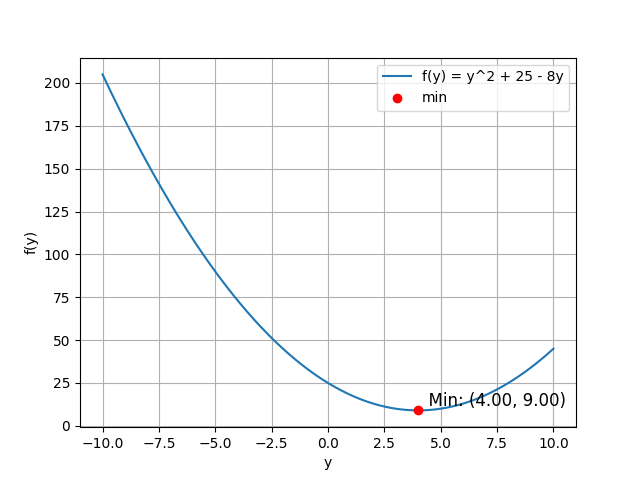
\includegraphics[width=\columnwidth]{figs/6.5.27.png}
   \caption{}
   \label{}
\end{figure}
\end{document}
